\documentclass[11pt]{article}
\usepackage[utf8]{inputenc}
\usepackage{amsfonts}
\usepackage{amsmath}
\usepackage{float}
\usepackage{tikz}
\usetikzlibrary{automata, positioning, arrows}
\tikzset{
  ->,
  >=stealth',
  node distance=3cm,
  every state/.style={thick, fill=gray!10},
  initial text=$ $,
}

\setlength{\parindent}{0em}
\setlength{\parskip}{1em}

\usepackage{geometry}
\geometry{
  a4paper,
  total={170mm,257mm},
  left=20mm,
  top=20mm,
}

\title{Problem Sheet 3}
\author{Rowan Saunders}
\begin{document}

\begin{titlepage}
	\maketitle
\end{titlepage}

\section{Regular Languages and Regular Expressions}
\subsection{Regular Operations}
The Union operation is defined as follows:

\begin{quote}
	For two languages $L_1, L_2 \subseteq \Sigma^\ast$, the \textbf{union} of
	these languages is denoted $L_1 \cup L_2$, and is defined analogously to sets.
	i.e. $L_1 \cup L_2$ contains all strings that are either members of $L_1$ or
	members $L_2$.
\end{quote}

The Concatenation operation is defined as follows:

\begin{quote}
	For two languages $L_1, L_2 \subseteq \Sigma^\ast$, their
	\textbf{concatenation}, which is denoted $L_1 \circ L_2$ (alternatively $L_1
		L_2$, is the language given by $L_1 \circ L_2 = \{uv | u \in L_1, v \in L_2 \}$
\end{quote}

An Concatenation example: Let the following both be languages defined over the alphabet $\{a, b\}$
\begin{align*}
	L_1 & = \{a^n | n = 1,2,3...\}, \\
	L_2 & = \{b^m | m = 1,2,3...\}
\end{align*}
Then:
$$ L_1 \circ L_2 = \{a^nb^m | n = 1,2,..., m=1,2,...\}$$
So
\begin{align*}
	aab & \in L_1 \circ L_2    \\
	bab & \notin L_1 \circ L_2
\end{align*}

Therefore, If $L=\{a^nb^m\}$, then $L^2 = L \circ L = \{a^nb^ma^lb^k\}$

The Kleene Star, or simply star operation is a unary operation, which has been
encountered before as $\Sigma^\ast$, which is the set of all strings in a given
alphabet $\Sigma$.

\begin{quote}
	Given a language $L$, the \textbf{Kleene star} is defined as:
	$$L^\ast=\{w_1w_2...w_n|w_i\in L, n = 0,1,...\}$$
	i.e.
	$$L^\ast=\{\varepsilon\} \cup L \cup L^2 \cup L^3 \cup ...$$
\end{quote}

A Kleene star example:
$$L = \{a^nb^m\}, L^\ast = \{a^{n_1}b^{m_1}a^{n_2}b^{m_2}...a^{n_k}b^{n_k}\}$$

If $L = \{a, b\}$ over $\Sigma = \{a, b\}$, then $L^\ast = \Sigma^\ast$

These three operations are called regular operations, because if you apply them
to regular languages, the results are regular too.

This represents the following Theorem:
\begin{quote}
	The class of regular languages is closed under the operations union,
	concatenation, and star. i.e. if $L_1$ and $L_2$ are regular languages, then
	the following languages are also regular:
	\begin{align*}
		\text{a)} & \quad L_1 \cup L_2                         \\
		\text{b)} & \quad L_1 \circ L_2                        \\
		\text{c)} & \quad L_1^\ast \quad (\text{and} L_2^\ast)
	\end{align*}
\end{quote}

The method for proving this theorem is to construct automata that accept these
languages $(L_1, L_2, a, b, c)$

\subsection{Proof that Union Operation is Regular}
Therefore, the proof that the Union operation is regular is as follows
\begin{quote}
	Assume we have regular languages $L_1$ and $L_2$. As they are regular, there
	must be finite automata $N_1$ and $N_2$ which accept these languages
	respectively. We wish to show that $L_1 \cup L_2$ is regular, and we do this
	by creating an NFA that accepts this language.
\end{quote}

The following NFAs can be constructed for $N_1$ (\emph{Figure \ref{fig:n1}}),
$N_2$ (\emph{Figure \ref{fig:n2}}) and $N_1 \cup N_2$ (\emph{Figure
	\ref{fig:n1un2}}). It makes no difference as to whether we use NFAs or DFAs,
however NFAs are often simpler to draw and document:

\begin{itemize}
	\item[]
	      \begin{figure}[H]
		      \centering
		      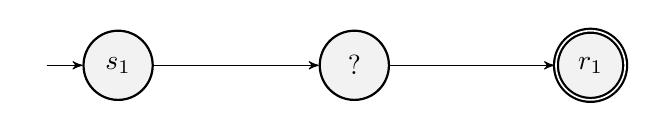
\begin{tikzpicture}
			      % states
			      \node[state, initial] (s) {$s_1$};
			      \node[state, right of=s] (q) {$?$};
			      \node[state, accepting, right of=q] (r) {$r_1$};

			      % transitions
			      \draw (s) edge[above] node{} (q)
			      (q) edge[above] node{} (r);

		      \end{tikzpicture}
		      \caption{$N_1$}
		      \label{fig:n1}
	      \end{figure}
	\item[]
	      \begin{figure}[H]
		      \centering
		      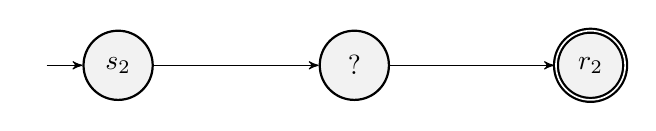
\begin{tikzpicture}
			      % states
			      \node[state, initial] (s) {$s_2$};
			      \node[state, right of=s] (q) {$?$};
			      \node[state, accepting, right of=q] (r) {$r_2$};

			      % transitions
			      \draw (s) edge[above] node{} (q)
			      (q) edge[above] node{} (r);

		      \end{tikzpicture}
		      \caption{$N_2$}
		      \label{fig:n2}
	      \end{figure}
	\item[]
	      \begin{figure}[H]
		      \centering
		      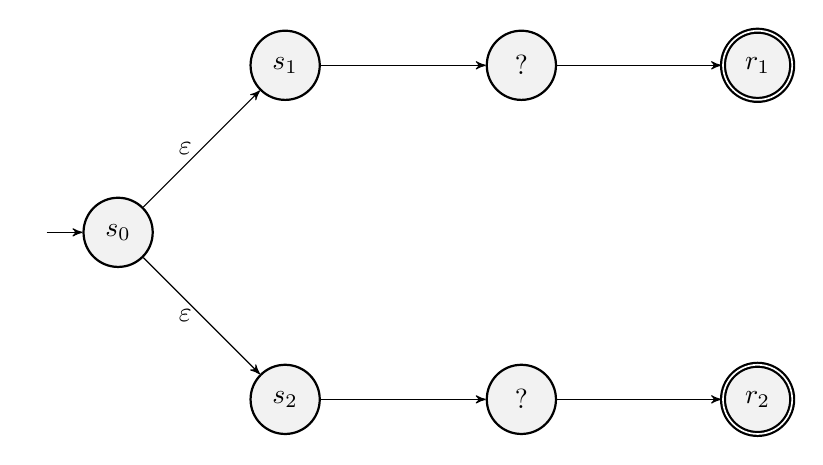
\begin{tikzpicture}
			      % states
			      \node[state, initial] (s0) {$s_0$};
			      \node[state, above right of=s0] (s1) {$s_1$};
			      \node[state, right of=s1] (q1) {$?$};
			      \node[state, accepting, right of=q1] (r1) {$r_1$};
			      \node[state, below right of=s0] (s2) {$s_2$};
			      \node[state, right of=s2] (q2) {$?$};
			      \node[state, accepting, right of=q2] (r2) {$r_2$};

			      % transitions
			      \draw (s0) edge[left] node{$\varepsilon$} (s1)
			      (s0) edge[left] node{$\varepsilon$} (s2)
			      (s1) edge[above] node{} (q1)
			      (q1) edge[above] node{} (r1)
			      (s2) edge[above] node{} (q2)
			      (q2) edge[above] node{} (r2);

		      \end{tikzpicture}
		      \caption{$N_1 \cup N_2$}
		      \label{fig:n1un2}
	      \end{figure}
\end{itemize}

Let $N_1=(Q_1,\Sigma,\delta_1,s_1,F_1)$ and $N_2=(Q_2,\Sigma,\delta_2,s_2,F_2)$
be non-deterministic finite automata which recognise $L_1$ and $L_2$
respectively.

We Construct $N=(Q,\Sigma,\delta,s_0,F)$ which recognises $L_1 \cup L_2$, where:

\begin{itemize}
	\item[] $Q = Q_1 \cup Q_2 \cup \{s_0\}$
	\item[] $\Sigma$ is the alphabet
	\item[] $\delta(q,a) =
		      \begin{cases}
			      \delta_1 (q,a) & q\in Q_1                         \\
			      \delta_2 (q,a) & q \in Q_2                        \\
			      \{s_1, s_2\}   & q=s_0 \text{ and } a=\varepsilon \\
			      \emptyset      & \text{otherwise}
		      \end{cases}$
	\item[] $s_0$ is the initial state
	\item[] $F = F_1 \cup F_2$
\end{itemize}

This completes the proof for closure of regular languages under the union
operation.

\newpage
\subsection{Proof Concatenation Operator is regular}
The proof that the Concatenation operation is regular is as follows
\begin{quote}
	Assume we have regular languages $L_1$ and $L_2$. As they are regular, there
	must be finite automata $N_1$ and $N_2$ which accept these languages
	respectively. We wish to show that $L_1 \circ L_2$ is regular, and we do this
	by creating an NFA that accepts this language.
\end{quote}

The following NFAs can be constructed for $N_1$ (\emph{Figure \ref{fig:concatn1}}),
$N_2$ (\emph{Figure \ref{fig:concatn2}}) and $N_1 \cup N_2$ (\emph{Figure
	\ref{fig:n1concatn2}}):

\begin{itemize}
	\item[]
	      \begin{figure}[H]
		      \centering
		      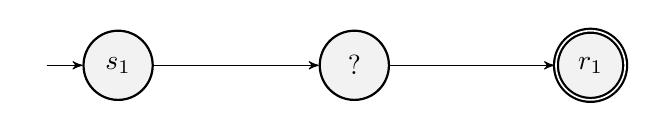
\begin{tikzpicture}
			      % states
			      \node[state, initial] (s) {$s_1$};
			      \node[state, right of=s] (q) {$?$};
			      \node[state, accepting, right of=q] (r) {$r_1$};

			      % transitions
			      \draw (s) edge[above] node{} (q)
			      (q) edge[above] node{} (r);

		      \end{tikzpicture}
		      \caption{$N_1$}
		      \label{fig:concatn1}
	      \end{figure}
	\item[]
	      \begin{figure}[H]
		      \centering
		      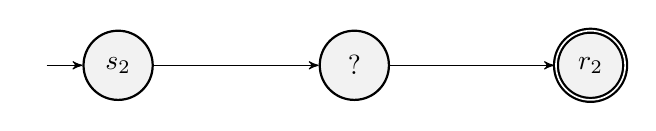
\begin{tikzpicture}
			      % states
			      \node[state, initial] (s) {$s_2$};
			      \node[state, right of=s] (q) {$?$};
			      \node[state, accepting, right of=q] (r) {$r_2$};

			      % transitions
			      \draw (s) edge[above] node{} (q)
			      (q) edge[above] node{} (r);

		      \end{tikzpicture}
		      \caption{$N_2$}
		      \label{fig:concatn2}
	      \end{figure}
	\item[]
	      \begin{figure}[H]
		      \centering
		      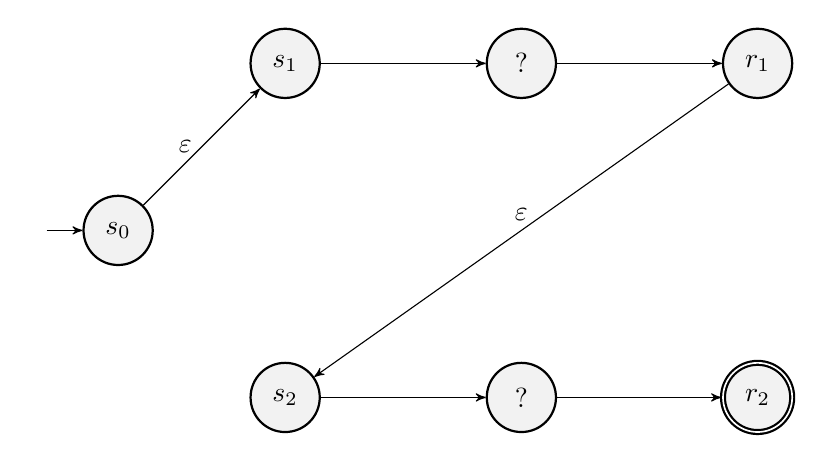
\begin{tikzpicture}
			      % states
			      \node[state, initial] (s0) {$s_0$};
			      \node[state, above right of=s0] (s1) {$s_1$};
			      \node[state, right of=s1] (q1) {$?$};
			      \node[state, right of=q1] (r1) {$r_1$};
			      \node[state, below right of=s0] (s2) {$s_2$};
			      \node[state, right of=s2] (q2) {$?$};
			      \node[state, accepting, right of=q2] (r2) {$r_2$};

			      % transitions
			      \draw (s0) edge[left] node{$\varepsilon$} (s1)
			      (r1) edge[above] node{$\varepsilon$} (s2)
			      (s1) edge[above] node{} (q1)
			      (q1) edge[above] node{} (r1)
			      (s2) edge[above] node{} (q2)
			      (q2) edge[above] node{} (r2);

		      \end{tikzpicture}
		      \caption{$N_1 \cup N_2$}
		      \label{fig:n1concatn2}
	      \end{figure}
\end{itemize}

Let $N_1=(Q_1,\Sigma,\delta_1,s_1,F_1)$ and $N_2=(Q_2,\Sigma,\delta_2,s_2,F_2)$
be non-deterministic finite automata which recognise $L_1$ and $L_2$
respectively.

We Construct $N=(Q,\Sigma,\delta,s_0,F)$ which recognises $L_1 \circ L_2$, where:

\begin{itemize}
	\item[] $Q = Q_1 \cup Q_2 \cup \{s_0\}$
	\item[] $\Sigma$ is the alphabet
	\item[] $\delta(q,a) =
		      \begin{cases}
			      \delta_1 (q,a) & q\in Q_1                         \\
			      \delta_2 (q,a) & q \in Q_2                        \\
			      \{s_1\}        & q=s_0 \text{ and } a=\varepsilon \\
			      \{s_2\}        & q=r_1 \text{ and } a=\varepsilon \\
			      \emptyset      & \text{otherwise}
		      \end{cases}$
	\item[] $s_0$ is the initial state
	\item[] $F = F_2$
\end{itemize}

This completes the proof for closure of regular languages under the
concatenate operation.

\newpage
\subsection{Proof Kleene Star Operator is regular}
The proof that the Kleene Star operation is regular is as follows
\begin{quote}
	Assume we have a regular language $L$. As this is regular, there
	must be finite automata $N$ which accepts this languages
	We wish to show that $L^\ast$ is regular, and we do this
	by creating an NFA that accepts this language.
\end{quote}

The following NFAs can be constructed for $N$ (\emph{Figure \ref{fig:n}})
and $N^\ast$ (\emph{Figure \ref{fig:nstar}}):

\begin{itemize}
	\item[]
	      \begin{figure}[H]
		      \centering
		      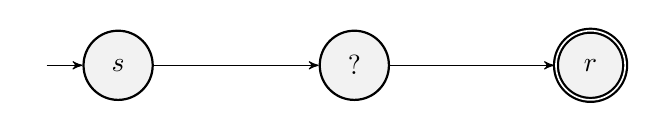
\begin{tikzpicture}
			      % states
			      \node[state, initial] (s) {$s$};
			      \node[state, right of=s] (q) {$?$};
			      \node[state, accepting, right of=q] (r) {$r$};

			      % transitions
			      \draw (s) edge[above] node{} (q)
			      (q) edge[above] node{} (r);

		      \end{tikzpicture}
		      \caption{$N$}
		      \label{fig:n}
	      \end{figure}
	\item[]
	      \begin{figure}[H]
		      \centering
		      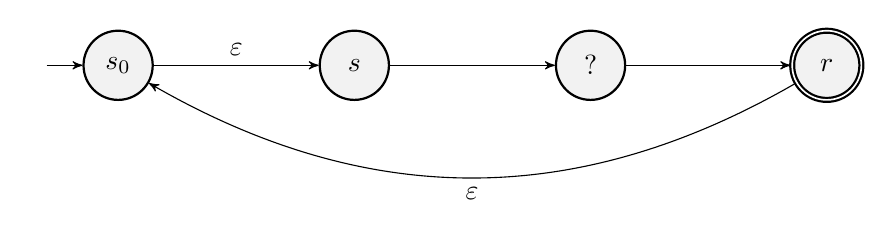
\begin{tikzpicture}
			      % states
			      \node[state, initial] (s0) {$s_0$};
			      \node[state, right of=s0] (s) {$s$};
			      \node[state, right of=s] (q) {$?$};
			      \node[state, accepting, right of=q] (r) {$r$};

			      % transitions
			      \draw (s) edge[above] node{} (q)
			      (q) edge[above] node{} (r)
			      (s0) edge[above] node{$\varepsilon$} (s)
			      (r) edge[bend left, below] node{$\varepsilon$} (s0);

		      \end{tikzpicture}
		      \caption{$N^\ast$}
		      \label{fig:nstar}
	      \end{figure}
\end{itemize}

Let $N=(Q,\Sigma,\delta,s,F)$ be non-deterministic finite automata which
recognises $L$.

We Construct
$N_{\text{star}}=(Q_{\text{star}},\Sigma,\delta_{\text{star}},s_0,F_{\text{star}})$
which recognises $L^\ast$, where:

\begin{itemize}
	\item[] $Q_{\text{star}} = Q \cup \{s_0\}$
	\item[] $\Sigma$ is the alphabet
	\item[] $\delta_{\text{star}}(q,a) =
		      \begin{cases}
			      \delta (q,a) & q\in Q                           \\
			      \{s_0\}      & q=r \text{ and } a=\varepsilon   \\
			      \{s\}        & q=s_0 \text{ and } a=\varepsilon \\
			      \emptyset    & \text{otherwise}
		      \end{cases}$
	\item[] $s$ is the initial state
	\item[] $F = \{r\}$
\end{itemize}

This completes the proof for closure of regular languages under the
Kleene Star operation.

\newpage
\section{Regular Expressions}
We define a regular expression recursively. This is also called an inductive
definition.

\begin{quote}
	Given an alphabet $\Sigma$ a \textbf{regular expression} is a string in the
	alphabet $\Sigma \cup \{(, ) , \varepsilon, \emptyset, \cup, \ast \}$, which
	meets the following rules:
	\begin{enumerate}
		\item $\emptyset, \varepsilon$ and $a \in \Sigma$ are regular expressions
		      (called \textbf{atomic regular expressions})
		\item if $\alpha$ and $\beta$ are regular expressions, then the following
		      expressions are regular expressions: $(\alpha \cup \beta), (\alpha\beta),
			      \alpha^\ast$
	\end{enumerate}
	Note that $\alpha\beta$ is the standard string concatenation.
\end{quote}

An example regular expression:

In the alphabet $\Sigma=\{a, b\}$, $(a \cup b) a^\ast$ is a regular expression.
Because:
\begin{itemize}
	\item[] $a$ and $b$ are regular expressions by rule 1
	\item[] So $(a \cup b)$ and $a^\ast$ are regular expressions by rule 2
	\item[] So $(a \cup b) a^\ast$ is a regular expressions by rule 2 again
\end{itemize}

$L(\alpha)$ is the language represented by regular expression $\alpha$

The language of a regular expression is defined by:
\begin{enumerate}
	\item $L(\emptyset) = \emptyset$
	\item $L(\varepsilon) = \varepsilon$
	\item $L(a) = a$ for every $a \in \Sigma$
	\item $L(\alpha \cup \beta) = L(\alpha) \cup L(\beta)$
	\item $L(\alpha\beta) = L(\alpha) \circ L(\beta)$
	\item $L(\alpha^\ast) = (L(\alpha))^\ast$
\end{enumerate}

For example, the language of $(a \cup b) a^\ast$:
\begin{itemize}
	\item[] $L((a \cup b) a^\ast)$
	\item[] $L((a \cup b)) \circ L(a^\ast)$ by rule 5
	\item[] $(L(a) \cup L(b)) \circ (L(a))^\ast$ by rule 4 and rule 6
	\item[] $(\{a\} \cup \{b\}) \circ \{a\}^\ast$ by rule 3
	\item[] $\{a, b\} \circ \{a^n | n \geq 0\}$ by regular operation definitions
\end{itemize}

We can write this as a single set in multiple ways. Here is one example:
$$(a \cup b) a^\ast = \{xa^n|x\in\{a,b\},n\geq0\}$$

We often drop redundant parenthesis, i.e the following left hand examples are
written as the right hand side:
\begin{align*}
	(a \cup (b \cup c)) & = a \cup b \cup c \\
	(a(bc))             & = abc
\end{align*}
There is no loss of meaning, as Union and Concatenation are associative.

Additionally, operations are always applied in a set order. The order of
precedence is:
\begin{enumerate}
	\item Star
	\item Concatenation
	\item Union
\end{enumerate}
Therefore:
\begin{align*}
	ab \cup c & \text{ means } (ab) \cup c \\
	ab^\ast   & \text{ means } a(b^\ast)
\end{align*}

We can use parentheses to change the order, so we could write:
$$a ( b \cup c)$$
$$(ab)^\ast$$


\subsection{Regular Expressions to Finite Automata}
We must now show that Regular Expressions are equivilent to DFA and NFAs, we can
do this with the following Theorem:
\begin{quote}
	\begin{itemize}
		\item[(a)] Any regular expression has an equivalent finite automaton
		\item[(b)] Any finite automaton has an equivalent regular expression
	\end{itemize}
\end{quote}

This Theorem has the following proof:
\begin{quote}
	First, construct NFAs for the atomic regular expressions $\emptyset,
		\varepsilon,$ and $a \in \Sigma$.

	These are as follows
	\begin{itemize}
		\item[]
		      \begin{figure}[H]
			      \centering
			      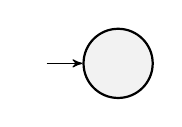
\begin{tikzpicture}
				      % states
				      \node[state, initial] (s) {};
			      \end{tikzpicture}
			      \caption{NFA that accepts the empty set $\emptyset$}
			      \label{fig:emptyset}
		      \end{figure}
		\item[]
		      \begin{figure}[H]
			      \centering
			      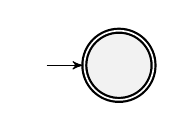
\begin{tikzpicture}
				      % states
				      \node[state, initial, accepting] (s) {};
			      \end{tikzpicture}
			      \caption{NFA that accepts the empty string $\varepsilon$}
			      \label{fig:emptystring}
		      \end{figure}
		\item[]
		      \begin{figure}[H]
			      \centering
			      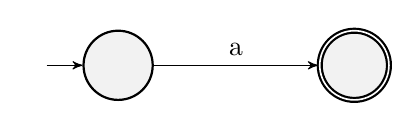
\begin{tikzpicture}
				      % states
				      \node[state, initial] (s) {};
				      \node[state, accepting, right of=s] (q) {};

				      % transitions
				      \draw (s) edge[above] node{a} (q);
			      \end{tikzpicture}
			      \caption{NFA that accepts a single letter in the alphabet $a \in \Sigma$}
			      \label{fig:ainsigma}
		      \end{figure}
	\end{itemize}
	Now, we can recursively use the earlier proofs of regular operations to build
	NFA which accept $\alpha \cup \beta$, $\alpha\beta$ and $\alpha^\ast$.
\end{quote}

\subsection{Converting Regular Expression into NFA}
We create a NFA from a regular expression by building the finite automata step
by step using the proofs described earlier for the regular operations.

For example for the regular expression $(a \cup b) a^\ast$:
\begin{itemize}
	\item[]
	      \begin{figure}[H]
		      \centering
		      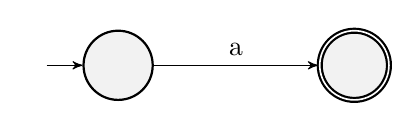
\begin{tikzpicture}
			      % states
			      \node[state, initial] (sa) {};
			      \node[state, accepting, right of=sa] (qa) {};

			      % transitions
			      \draw (sa) edge[above] node{a} (qa);
		      \end{tikzpicture}
		      \caption{NFA to accept $a \in \Sigma$}
		      \label{fig:re2nfa1}
	      \end{figure}
	\item[]
	      \begin{figure}[H]
		      \centering
		      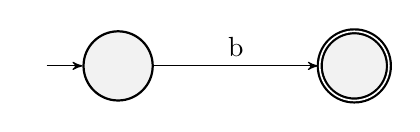
\begin{tikzpicture}
			      % states
			      \node[state, initial] (sb) {};
			      \node[state, accepting, right of=sb] (qb) {};

			      % transitions
			      \draw (sb) edge[above] node{b} (qb);
		      \end{tikzpicture}
		      \caption{NFA to accept $b \in \Sigma$}
		      \label{fig:re2nfa2}
	      \end{figure}
	\item[]
	      \begin{figure}[H]
		      \centering
		      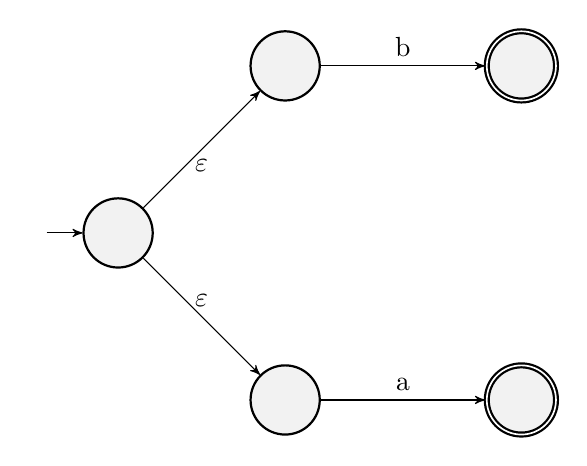
\begin{tikzpicture}
			      % states
			      \node[state, initial] (s0) {};
			      \node[state, below right of=s0] (sa) {};
			      \node[state, accepting, right of=sa] (qa) {};
			      \node[state, above right of=s0] (sb) {};
			      \node[state, accepting, right of=sb] (qb) {};

			      % transitions
			      \draw (s0) edge[above] node{$\varepsilon$} (sa)
			      (s0) edge[below] node{$\varepsilon$} (sb)
			      (sa) edge[above] node{a} (qa)
			      (sb) edge[above] node{b} (qb);
		      \end{tikzpicture}
		      \caption{NFA to accept $a \cup b$}
		      \label{fig:re2nfa3}
	      \end{figure}
	\item[]
	      \begin{figure}[H]
		      \centering
		      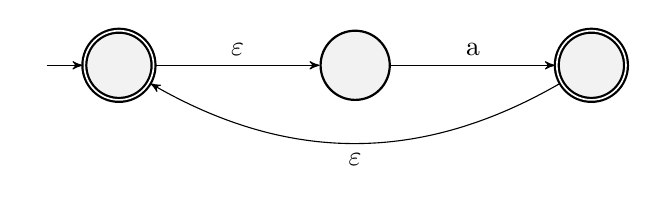
\begin{tikzpicture}
			      % states
			      \node[state, accepting, initial] (s0) {};
			      \node[state, right of=s0] (sa) {};
			      \node[state, accepting, right of=sa] (qa) {};

			      % transitions
			      \draw (s0) edge[above] node{$\varepsilon$} (sa)
			      (qa) edge[bend left, below] node{$\varepsilon$} (s0)
			      (sa) edge[above] node{a} (qa);
		      \end{tikzpicture}
		      \caption{NFA to accept $a^\ast$}
		      \label{fig:re2nfa4}
	      \end{figure}
	\item[]
	      \begin{figure}[H]
		      \centering
		      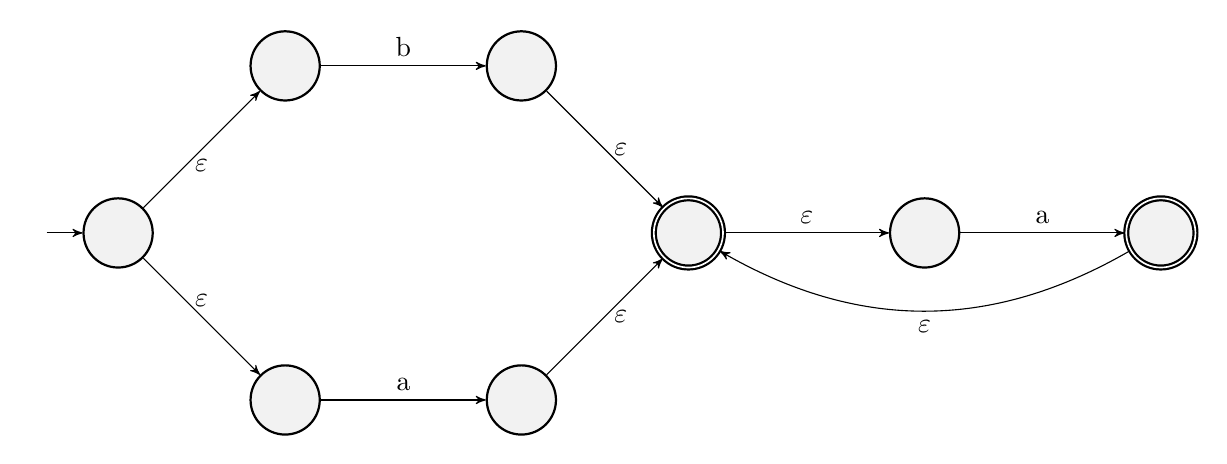
\begin{tikzpicture}
			      % states
			      \node[state, initial] (s0) {};
			      \node[state, below right of=s0] (sa) {};
			      \node[state, right of=sa] (qa) {};
			      \node[state, above right of=s0] (sb) {};
			      \node[state, right of=sb] (qb) {};

			      \node[state, accepting, below right of=qb] (ss) {};
			      \node[state, right of=ss] (ssa) {};
			      \node[state, accepting, right of=ssa] (qsa) {};

			      % transitions
			      \draw (s0) edge[above] node{$\varepsilon$} (sa)
			      (s0) edge[below] node{$\varepsilon$} (sb)
			      (sa) edge[above] node{a} (qa)
			      (sb) edge[above] node{b} (qb)
						(qa) edge[right] node{$\varepsilon$} (ss)
						(qb) edge[right] node{$\varepsilon$} (ss)
			      (ss) edge[above] node{$\varepsilon$} (ssa)
			      (qsa) edge[bend left, below] node{$\varepsilon$} (ss)
			      (ssa) edge[above] node{a} (qsa);
		      \end{tikzpicture}
					\caption{NFA to accept $(a \cup b) \circ a^\ast$}
		      \label{fig:re2nfa5}
	      \end{figure}
\end{itemize}

\subsection{Converting Finite Automata into Regular Expressions}

\end{document}
